% Created 2021-05-28 Fri 19:41
% Intended LaTeX compiler: pdflatex
\documentclass[a4paper,11pt]{article}
\usepackage[utf8]{inputenc}
\usepackage[T1]{fontenc}
\usepackage{graphicx}
\usepackage{grffile}
\usepackage{longtable}
\usepackage{wrapfig}
\usepackage{rotating}
\usepackage[normalem]{ulem}
\usepackage{amsmath}
\usepackage{textcomp}
\usepackage{amssymb}
\usepackage{capt-of}
\usepackage{hyperref}
\usepackage{geometry}
\geometry{a4paper, left=20mm, top=20mm}
\author{Diego Joshua Martínez Pineda (diem@itu.dk)}
\date{\today}
\title{Software Reconstruction}
\hypersetup{
 pdfauthor={Diego Joshua Martínez Pineda (diem@itu.dk)},
 pdftitle={Software Reconstruction},
 pdfkeywords={},
 pdfsubject={},
 pdfcreator={Emacs 27.2 (Org mode 9.4.4)}, 
 pdflang={English}}
\begin{document}

\maketitle

\section{Introduction}
\label{sec:orgc794855}

For this assignment, the \href{https://scrapy.org/}{Scrapy framework} for creating web crawlers/scrappers was chosen as a case of study. The aim was to obtain insights on the open source codebase of Scrapy, therefore a tool for visualizing the dependencies between modules and possibly interacting with the desired layout was developed. Such a visualization corresponds to a polymetric view as discussed on class.

The developed tool can be seen \textbf{live} here: \url{https://mynjj.github.io/architecture-reconstruction/index.html}

\section{Rationale}
\label{sec:orgd3dc161}

\label{rationale}
A polymetric view was reconstructed out of Scrapy's open source code base. The implemented polymetric view is based on the module view of the system and allows for visualization of the module dependencies, while also taking into account the cyclotomic complexity of the modules.

Furthermore a tool surrounding such view was also developed. The same guiding principles behind \cite{poly}, that is, allowing the human brain to grasp structure out of large systems via visual representations, is followed. However, due to the constant evolving nature of software and human-software interactions it's to be expected for tools to have changed since 2003, this was therefore taken advantage from, using current web technologies more interactive than a static image.

The concept of how interactive manipulations may allow for creative thinking surrounding a problem has been explored, quite interestingly by Bret Victor \cite{dynamic} \cite{deadfish}. I find important for software tools and representation of information to exploit everything that software has to offer, instead of it being only a static representation of data.

This inspired the former proof of concept (POC), a tool reconstructing a Module View from the software architecture of the framework, enhancing it with more information, such as the modules' McCabe complexity.

Furthermore, this exploratory tool is expected to be used with an intent, and the manipulations should be in regards of the questions expected to be solved with it. The exploratory tool should then be an aid for solving questions and a framework under which to think problems in your domain, much similar to the Glamorous Toolkit shown \cite{glamour} on our lecture. There is however always the risk that once a tool is developed, the usage of the tool becomes its creative constraint and the user starts thinking in terms of the tool instead of creatively.

Much has been said around what makes a tool useful, and the principles under which one should approach tool development. The former POC doesn't explore much on this, only on interactivity and how it could be useful.

\section{The tool}
\label{sec:org8d120f4}
The tool was developed roughly on 4 days, sacrificing proper software development practices, in favor of speed of getting the desired results. 

The source code for the tool can be seen here \href{https://github.com/mynjj/architecture-reconstruction}{https://github.com/mynjj/architecture-reconstruction}.

A Python script using the modules \texttt{ast} and \texttt{mccabe} traverses the code through entry points, reading dependencies recursively (DFS) and computing McCabe complexities along the way. This is later flattened into a JSON file that a React/D3 application reads.

Much improvements should be made for this to be a useful tool for source code exploration, however, as stated before, the POC only explored how interactivity can fit and be exploited on the concept of a software architecture view. The produced views resemble polymetric views.

One should also note that only \texttt{import} relations are explored, and that more complex interactions possible due to Python's dynamic nature can remain uncaptured.

\section{Results}
\label{sec:org885a321}


\subsection{Overview of the tool}
\label{sec:org76949e1}

The tool is composed of 3 main sections:

\begin{enumerate}
\item Configuration. On the right column, top section, one can configure different settings for the resulting view. Like wether or not to show names on the modules, the external dependencies or pick specific modules to show.
\item Diagram view. The result of the configuration with the relations extracted form the code base are shown here.
\item Module details. When one clicks a graph node representing a module a dark transparent overlay shows on top where one can explore the artifact and complexity that the module has.
\item Trivia. On the right column, bottom section, several ``trivia'' information is shown, like the most complex files and artifacts on the code base.
\end{enumerate}

See figure \ref{ui} for an overview.

Among the features that proved useful was adding 

\begin{figure}
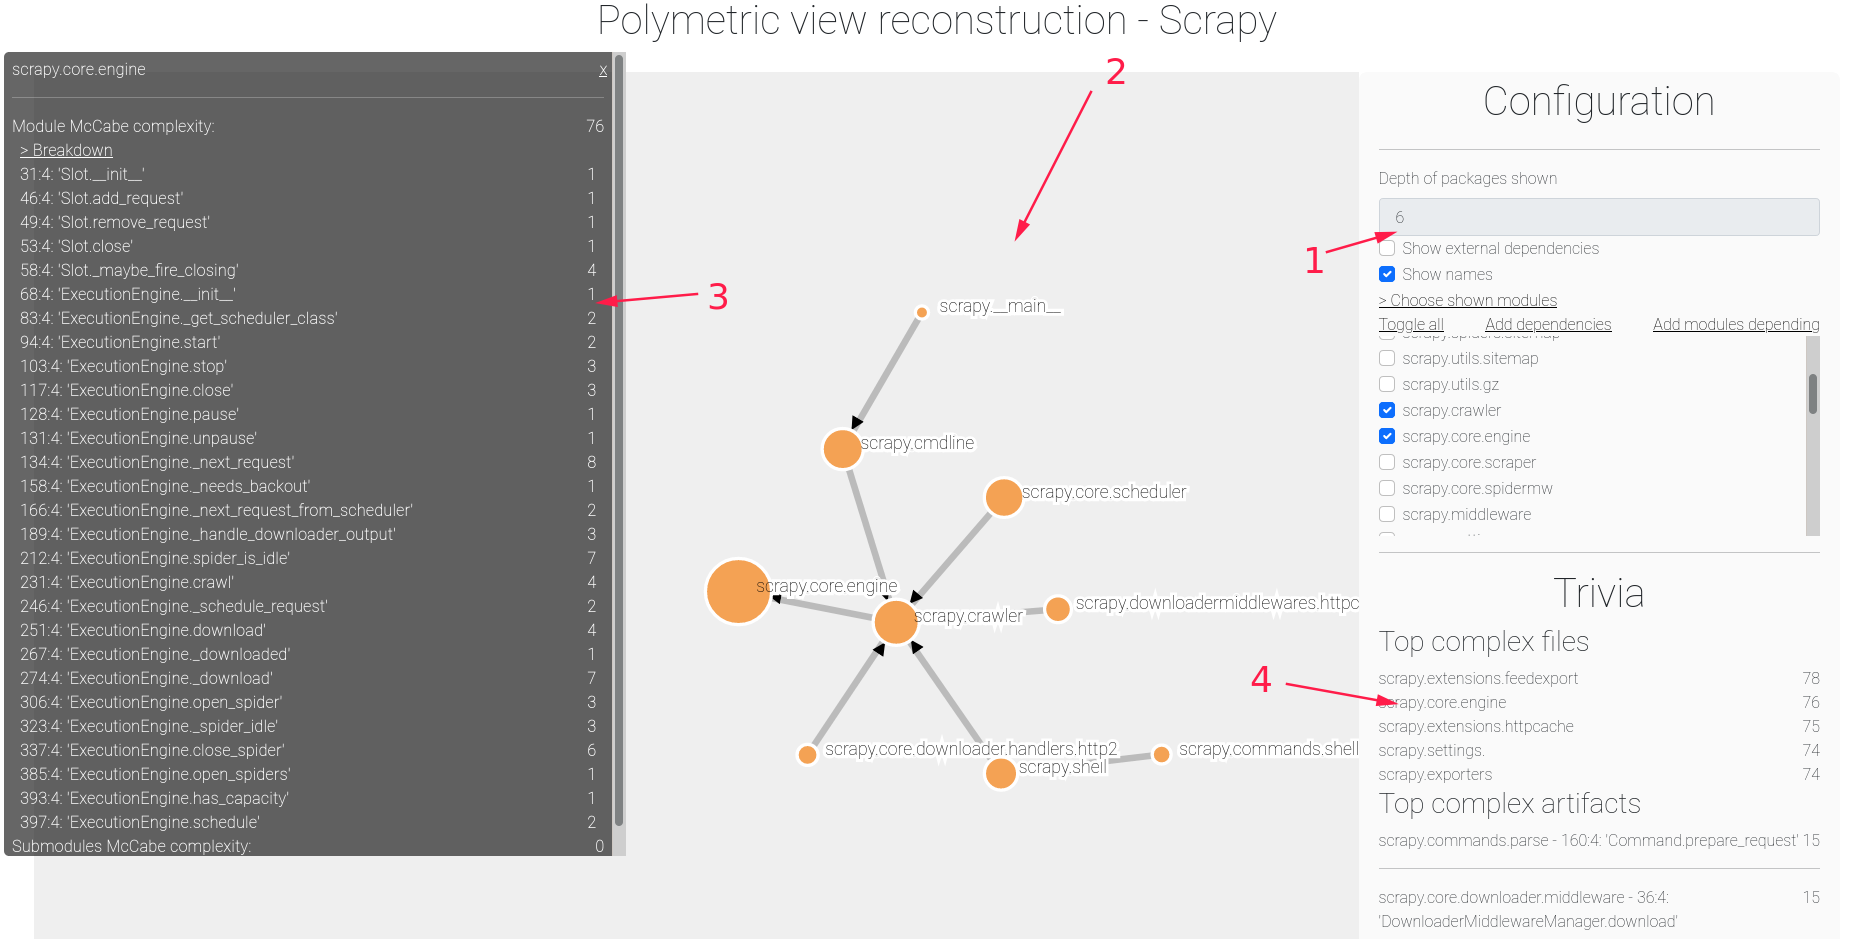
\includegraphics[width=.9\linewidth]{../screenshots/ui.png}
\caption{Interface overview}
\label{ui}
\end{figure}


\subsection{Explorations}
\label{sec:org7929cba}
As stated on section \ref{rationale}, we explored with intent, and the following questions were addressed:

\subsubsection{What is the most complex file? How careful should one be before changing it? Is refactoring it feasible?}
\label{sec:org80abbec}
On the ``Trivia'' section of the tool, one can see \texttt{scrapy.extensions.feedexport} as the most complex.

By setting ``Depth of packages shown'' to 6, selecting ``Choose shown modules'', clicking ``Toggle all'', and only selecting this file, one can add the modules depending on the currently selected by clicking ``Add dependents''. See figure \ref{feedexport}.

This shows that there's no module depending on it, and it's instead used directly by the consumer of the framework, it could then be refactored or splitted across its different units of functionality if this deemed useful with only the consideration of breaking changes for its API.

In particular this module, as explained on Scrapy's doumentation, deals with exporting scrapped data into different formats and storages. If one clicks the node, one can see that there's no particularly complex unit, but it's instead a large file. This is in intself not a bad thing, however if related functionality is in the project's roadmap and reuse of this sections might be useful, improvements here could be considered.

We can further explore the second most complex file: \texttt{scrapy.core.engine} according to the ``Trivia'' section. Similarly by clicking repeatedly ``Add dependents''. One can see that \texttt{scrapy.crawler} depends on it, and that this in turns has several entry points as dependencies, like the \texttt{scrapy.cmdline} or the \texttt{scrapy.core.scheduler}.

See \href{https://github.com/mynjj/architecture-reconstruction/tree/main/screenshots/getting-deps.gif}{on this link} an animation of this process.

This reflects that changes on this file should be made with more care on the implications they may have. The source of complexity for this module is also not because of a particularly complex artifact, but because of its length and functionality encompassed. See figure \ref{coreengine}.

\begin{figure}
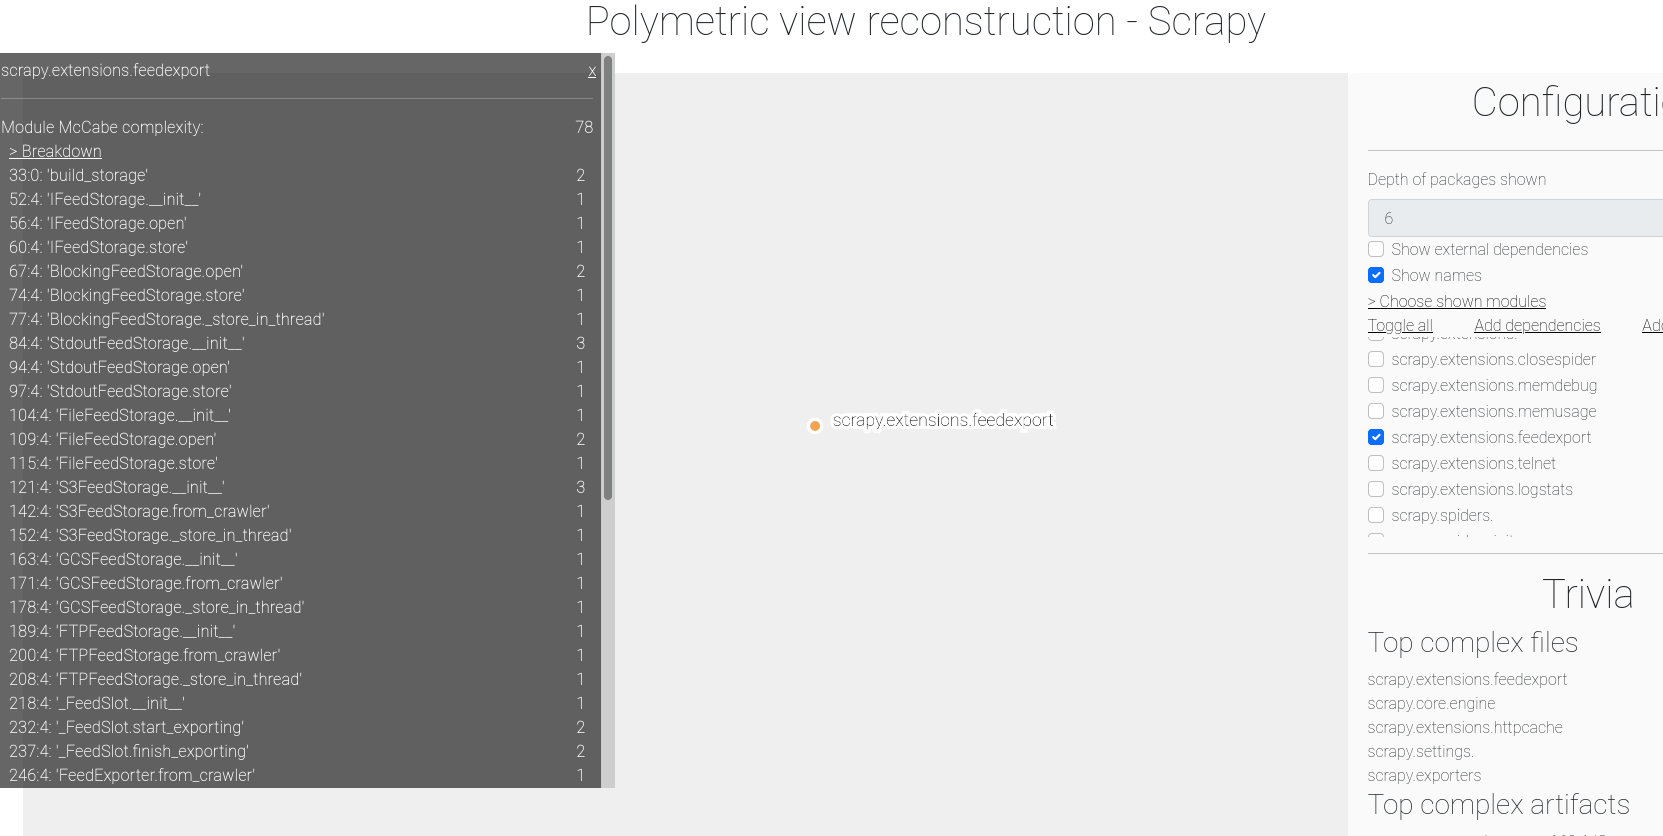
\includegraphics[width=.9\linewidth]{../screenshots/feedexport.png}
\caption{Dependency expansion of \texttt{scrapy.extensions.feedexport}}
\label{feedexport}
\end{figure}

\begin{figure}
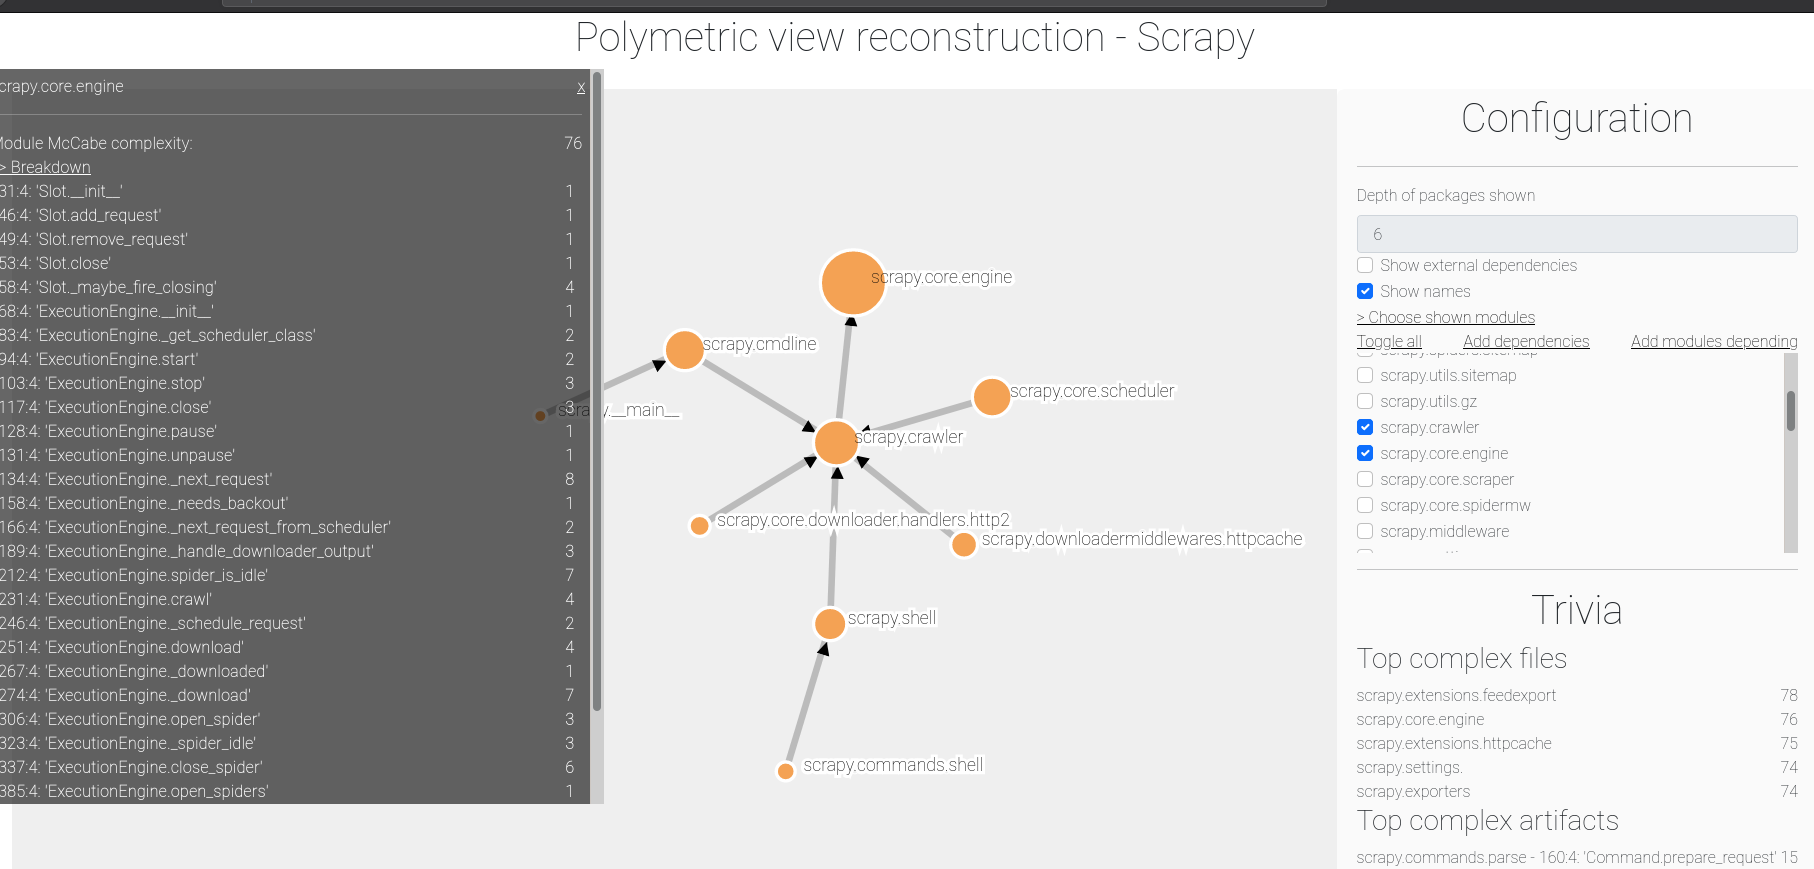
\includegraphics[width=.9\linewidth]{../screenshots/coreengine.png}
\caption{Dependency expansion of \texttt{scrapy.core.engine}}
\label{coreengine}
\end{figure}

\subsubsection{Where is the most complex method? Is it critical? Is refactoring worth it?}
\label{sec:orgdb2f33a}
Also on the trivia section, one can see that the method \texttt{prepare\_request} of the class \texttt{Command} on the module \texttt{scrapy.commands.parse}, has a cyclotomic complexity of 15.

The same dependencies analysis as before shows that no module depends on it, and that it's an entry point of the system. However if maintainability of this process is required, refactoring might be useful. We can argue that this function while complex does what required well, this is reflected on the repository history of this particular file \url{https://github.com/scrapy/scrapy/blame/master/scrapy/commands/parse.py} , where the last change on this method was 10 months ago, and that only ocassional commits are done on this section.

\subsubsection{External dependencies}
\label{sec:org3a2966d}
With ``Depth of packages shown'' set to 2, and seeing external dependencies, one can see most of the external dependencies as requirements of \texttt{scrapy.utils}. This shows that somehow a connection of external dependencies with the internal code of the project is provided by modules under \texttt{scrapy.utils}. I believe this to be in general a good idea. See figure \ref{deps}.

\begin{figure}
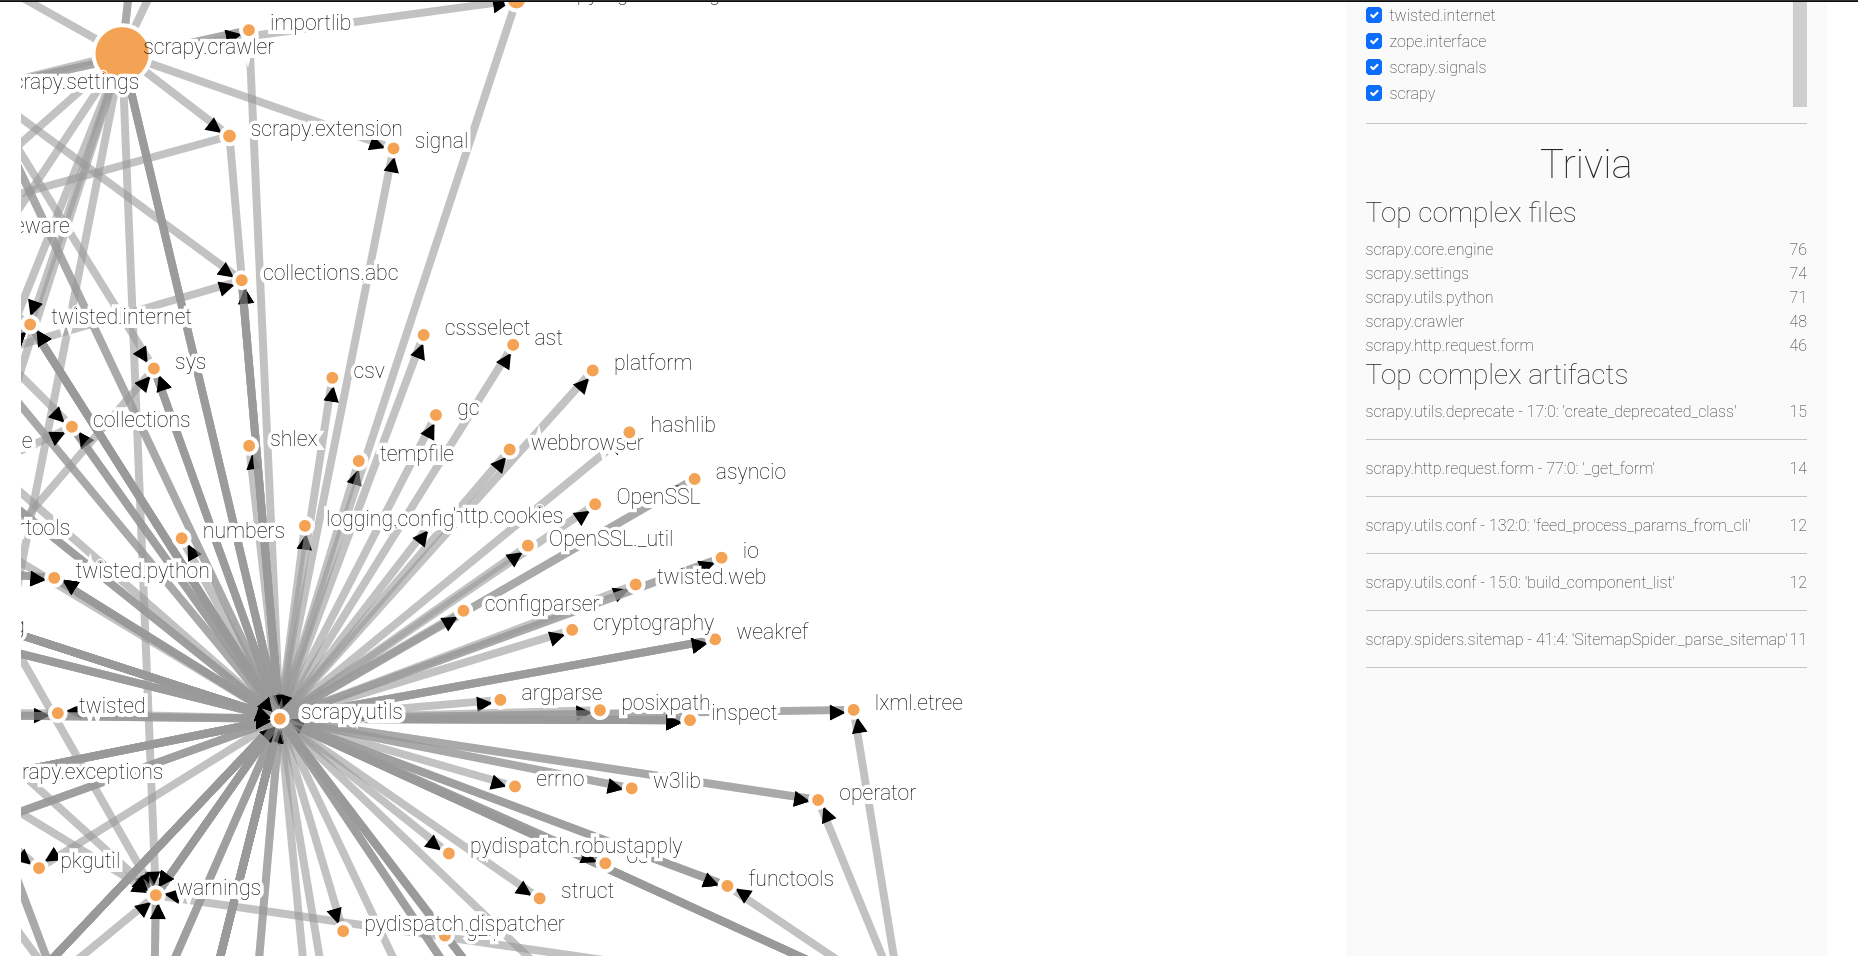
\includegraphics[width=.9\linewidth]{../screenshots/external_deps.png}
\caption{Visualizing external dependencies}
\label{deps}
\end{figure}

\section{Future}
\label{sec:orgcad505c}

On a final related note, while having valuable insights of the code base with this visualization tool, one may question the value it provides. And whether it's worth to have this kind of project on the side which in turn will imply mantaining a different code base. For instance, while this project was done with React and D3 (popular on 2021 for interactive software and visualizations), we can't for sure predict the future of interactions, and for a prolonged life of this project, its value must be scattered across the right abstractions, sufficiently decoupled, but still providing value.

This could only be determined by the specific use-case. One can even argue that much of the recent focus and development is on this regard, frameworks and languages can also be seen as tools, and the former React and D3 provide powerful abstractions without being too opinionated on the principles its users should follow, making them very versatile. It's my belief that this is an important part of its success. Versatility and lack of constraints allow for creativity, that might be the reason why for me, nothing beats pen and paper for my creative thinking, although this last approach doesn't scale well.

The usage of dynamic abstractions for data visualizations is also something popular with recent focus on tools like PowerBI, where one can leverage a lot of abstractions for several data sources and multiple visualization engines while being greatly customizable. It could even be the case that it may prove useful in visualizing code bases as well.

\section{Conclusions}
\label{sec:org64d87fd}

The tool can aid to visually have a perspective on some questions, however much is lacking for it to be a more insightful tool. Little changes on the code should be required to make this a tool applicable for any Python code base, however it's unclear if this is worth it, whether or not this provides the right abstractions that don't over-constraint the user.

Most likely any project that requires this kind of visual insight would require its particular set of assumptions/metrics/outcomes, and this should always be in line with the goals and the drivers for the desire of such a tool. This makes it more likely for it to be a personalized tool instead of a mytical software visualization silver bullet. This is even more true now that systems are scattered across several code bases in the form of micro-services.

\begin{thebibliography}{9}
\bibitem{poly}\textit{Symphony: View-Driven Software Architecture Reconstruction}, Deursen, Hofmesiter et.al.

\bibitem{dynamic}\textit{Drawing Dynamic Visualizations}: Bret Victor, \href{https://vimeo.com/66085662}{https://vimeo.com/66085662}

\bibitem{deadfish}\textit{Stop drawing dead fish}: Bret Victor, \href{https://vimeo.com/64895205}{https://vimeo.com/64895205}

\bibitem{glamour} Glamourous Toolkit, \href{https://gtoolkit.com/}{https://gtoolkit.com/}
\end{thebibliography}
\end{document}
